\section{Подобие треугольников}

\paragraph{Предварительные понятия.}\label{1938/156}
В окружающей нас жизни часто встречаются фигуры, имеющие различные размеры, но одинаковую форму.
Таковы, например, одинаковые фотографии одного и того же лица, изготовленные в различных размерах, или планы здания или целого города, вычерченные в различных масштабах. 
Такие фигуры принято называть подобными.
Умение измерять длины отрезков позволяет точно определить понятие о геометрическом подобии фигур и дать способы изменения размера фигуры без изменений её формы.

Изучение подобия фигур мы начнём с простейшего случая, именно с подобия треугольников.

\paragraph{}\label{1938/158}
\so{Определение}.
\emph{Два треугольника называются \rindex{подобные!треугольники}подобными, если:
1) углы одного соответственно равны углам другого и 
2) стороны одного пропорциональны соответственным сторонам другого.}

\begin{figure}[h!]
\centering
\includegraphics{mppics/ris-extra-4}
\caption{}\label{extra/ris-4}
\end{figure}

Подобие треугольников обозначается знаком $\sim$;
например, $\triangle ABC\z\sim \triangle DEF$ означает, что треугольники $ABC$ и $DEF$ подобны.
При этом принято выписывать соответственные вершины треугольников в том же порядке;
то есть  $\triangle ABC\sim \triangle DEF$ обычно означает, что 
\[\angle A=\angle D,\quad
 \angle B=\angle E,\quad
 \angle C=\angle F
\]
и
\[\frac{AB}{DE}=\frac{BC}{EF}=\frac{AC}{DF}.\]

То, что подобные треугольники существуют, показывает следующая лемма\footnote{Леммой называется вспомогательная теорема, которая излагается для того, чтобы при её помощи доказать следующую за ней теорему.}.

\paragraph{}\label{1938/159}
\so{Лемма}.
\textbf{\emph{Прямая}} ($EF$, рис.~\ref{1938/ris-169}), \textbf{\emph{параллельная какой-нибудь стороне}} ($AC$) \textbf{\emph{треугольника}} ($ABC$), \textbf{\emph{отсекает от него треугольник}} ($DBE$), \textbf{\emph{подобный данному.}}

Пусть в треугольнике $ABC$ прямая $DE$ параллельна стороне $AC$.
Требуется доказать, что $\triangle DBE\sim \triangle ABC$.

Предстоит доказать, во-первых, равенство соответственных углов и, во-вторых, пропорциональность соответственных сторон треугольников $ABC$ и $DBE$.

1.
Углы треугольников соответственно равны, так как угол $B$ у них общий, а $\angle D = \angle A$ и $\angle E= \angle C$, как соответственные углы при параллельных $DE$ и $AC$ и секущих $AB$ и $CB$.

2.
Докажем, что стороны $\triangle DBE$ пропорциональны соответственным сторонам $\triangle ABC'$, то есть что
\[\frac{BD}{BA}=\frac{BE}{BC}=\frac{DE}{AC}.\]

Для этого рассмотрим отдельно следующие два случая:

1.
\so{Стороны $AB$ и $BD$ имеют общую меру}.

\begin{wrapfigure}[13]{r}{51mm}
\centering
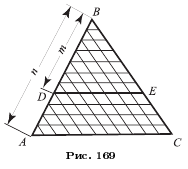
\includegraphics{mppics/ris-169}
\caption{}\label{1938/ris-169}
\end{wrapfigure}

Разделим $AB$ на части, равные этой общей мере.
Тогда $BD$ разделится на целое число таких частей.
Пусть этих частей содержится $m$ в $BD$ и $n$ в $AB$.
Проведём из точек деления ряд прямых, параллельных $AC$, и другой ряд прямых, параллельных $BC$.
Тогда $BE$ и $BC$ разделятся на равные части (§~\ref{1938/95}), которых будет $m$ в $BE$ и $n$ в $BC$.
Точно так же $DE$ разделится на $m$ равных частей, а $AC$ на $n$ равных частей, причём части $BE$ равны частям $AC$ (как противоположные стороны параллелограммов).
Теперь очевидно, что
\begin{align*}
\frac{BD}{BA}&=\frac mn,
&
\frac{BE}{BC}&=\frac mn,
&
\frac{DE}{AC}&=\frac mn.
\end{align*}



Следовательно
\[\frac{BD}{BA}=\frac{BE}{BC}=\frac{DE}{AC}.\]

2. \so{Стороны} $AB$ и $BD$ \so{не имеют общей меры} (рис.~\ref{1938/ris-170}).

Найдём приближённые значения каждого из отношений $\frac{BD}{BA}$ и $\frac{BE}{BC}$, сначала с точностью до $\tfrac1{10}$;
затем до $\tfrac1{100}$ и далее будем последовательно повышать степень точности в 10 раз.

\begin{wrapfigure}{r}{45mm}
\centering
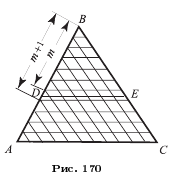
\includegraphics{mppics/ris-170}
\caption{}\label{1938/ris-170}
\end{wrapfigure}

Для этого разделим сторону $AB$ сначала на 10 равных частей и через точки деления проведём прямые, параллельные $AC$.
Тогда сторона $BC$ разделится также на 10 равных частей.
Предположим, что $\tfrac1{10}$ доля $AB$ укладывается в $BD$ более $m$
раз, причём остаётся остаток, меньший $\tfrac1{10}AB$.

Тогда, как видно из рис.~\ref{1938/ris-170}, $\tfrac1{10}$ доля $BC$ укладывается в $BE$ также $m$ раз и остаётся остаток, меньший $\tfrac1{10}BC$.
Следовательно, с точностью до $\tfrac1{10}$ имеем:
\[\frac{BD}{AB}=\frac{m}{10}; 
\quad
\frac{BE}{BC}=\frac{m}{10}\]
Далее, разделим $AB$ на 100 равных частей и предположим, что $\tfrac1{100}AB$ укладывается $m_1$ раз в $BD$.
Проводя опять через точки деления прямые, параллельные $AC$, убеждаемся, что $\tfrac1{100}BC$ укладывается в $BE$ также $m_1$ раз.
Поэтому с точностью до $\tfrac1{100}$ имеем:
\[\frac{BD}{AB}=\frac{m_1}{100}; 
\quad
\frac{BE}{BC}=\frac{m_1}{100}\]

Повышая далее степень точности в $10,100,\dots$ раз, убеждаемся, что приближённые значения соотношений $\frac{BD}{BA}$ и $\frac{BE}{BC}$, вычисленные с произвольной, но одинаковой десятичной точностью, равны.
Следовательно, значения этих отношений выражаются одной и той же бесконечной десятичной дробью;
значит
\[\frac{BD}{BA}=\frac{BE}{BC}.\]

Точно так же, проводя через точки деления стороны $AB$ прямые, параллельные стороне $BC$, найдём, что
\[\frac{BD}{BA}=\frac{DE}{AC}.\]

Таким образом, и в этом случае имеем:
\[\frac{BD}{BA}=\frac{BE}{BC}=\frac{DE}{AC}.\]


\paragraph{}\label{1938/160}
\so{Замечание}:
Доказанные соотношения представляют собой три следующие пропорции:
\[\frac{BD}{BA}=\frac{BE}{BC};
\quad
\frac{BD}{BA}=\frac{DE}{AC};
\quad
\frac{BE}{BC}=\frac{DE}{AC}.\]
Переставив в них средние члены, получим:
\[\frac{BD}{BE}=\frac{BA}{BC};
\quad
\frac{BD}{DE}=\frac{BA}{AC};
\quad
\frac{BE}{DE}=\frac{BC}{AC}.\]

Таким образом, если в треугольниках стороны пропорциональны, то отношение любых двух сторон одного треугольника равно отношению соответственных сторон другого треугольника.

\subsection*{Признаки подобия треугольников}

\paragraph{}\label{1938/161}
\so{Теоремы}.
\textbf{\emph{Если в двух треугольниках:}}

1) \textbf{\emph{два угла одного треугольника соответственно равны двум, углам, другого}} или

2) \textbf{\emph{две стороны одного треугольника пропорциональны двум сторонам другого и углы, лежащие между этими сторонами, равны}} или

3) \textbf{\emph{если три стороны одного треугольника пропорциональны трём сторонам другого, то такие треугольники подобны.}}

1) Пусть $ABC$ и $A_1B_1C_1$ (рис.~\ref{1938/ris-171}) будут два треугольника, у которых $\angle A = \angle A_1$, $\angle B=\angle B_1$ и, следовательно, $\angle C=\angle C_1$.
Требуется доказать, что такие треугольники подобны.

\begin{figure}[h!]
\centering
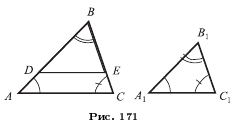
\includegraphics{mppics/ris-171}
\caption{}\label{1938/ris-171}
\end{figure}

Отложим на $AB$ отрезок $BD$, равный $A_1B_1$, и проведём $DE\z\parallel AC$.
Согласно доказанной выше лемме, $\triangle DBE\sim\triangle ABC$.

С другой стороны, $\triangle DBE= \triangle A_1B_1C_1$, потому что у них:
$BD\z=A_1B_1$ (по построению), $\angle B=\angle B_1$ (по условию) и $\angle D \z= \angle A_1$ (потому что $\angle D = \angle A$ и $\angle A = \angle A_1$).
Но очевидно, что если из двух равных треугольников один подобен третьему, то и другой ему подобен;
следовательно, 
\[\triangle A_1B_1C_1\sim\triangle ABC.\]

2) Пусть в треугольниках $ABC$ и $A_1B_1C_1$ (рис.~\ref{1938/ris-172}) дано.

\[\angle B=\angle B_1
\quad
\text{и}
\quad
\frac{AB}{A_1B_1}=\frac{BC}{B_1C_1}.\eqno(1)\]

\begin{figure}[h!]
\centering
\includegraphics{mppics/ris-172}
\caption{}\label{1938/ris-172}
\end{figure}

Требуется доказать, что такие треугольники подобны.
Отложим снова на $AB$ отрезок $BD$, равный $A_1B_1$, и проведём $DE\parallel AC$.
Тогда получим вспомогательный $\triangle DBE$, подобный $\triangle ABC$.
Докажем, что он равен $\triangle A_1B_1C_1$.
Из подобия треугольников $ABC$ и $DBE$ следует:
\[\frac{AB}{DB}=\frac{BC}{BE}\eqno(2)\]

Сравнивая эту пропорцию с данной пропорцией (1), замечаем, что первые отношения обеих пропорций одинаковы ($DB\z=A_1B_1$ по построению);
следовательно, остальные отношения этих пропорций также равны, то есть 
\[\frac{BC}{B_1C_1}=\frac{BC}{BE}\]
Но если в пропорции предыдущие члены равны, то должны быть равны и последующие члены, значит
\[B_1C_1=BE.\]

Теперь видим, что треугольники $DBE$ и $A_1B_1C_1$ имеют по равному углу ($\angle B=\angle B_1$), заключённому между соответственно равными сторонами;
значит, эти треугольники равны.
Но $\triangle DBE$ подобен $\triangle ABC$, поэтому и $\triangle A_1B_1C_1$ подобен $\triangle ABC$.

3) Пусть в треугольниках $ABC$ и $A_1B_1C_1$ (рис.~\ref{1938/ris-173}) дано:
\[
\frac{AB}{A_1B_1}=\frac{BC}{B_1C_1}=\frac{AC}{A_1C_1}.\eqno(1)\]
Требуется доказать, что такие треугольники подобны.

\begin{figure}[h!]
\centering
\includegraphics{mppics/ris-173}
\caption{}\label{1938/ris-173}
\end{figure}

Сделав построение такое же, как и прежде, покажем, что $\triangle DBE\z=\triangle A_1B_1C_1$.
Из подобия треугольников $ABC$ и $BDE$ следует:
\[\frac{AB}{DB}=\frac{BC}{BE}=\frac{AC}{DE}\eqno(2)\]

Сравнивая этот ряд отношений с данным рядом (1), замечаем, что первые отношения у них равны, следовательно, и остальные отношения равны, и потому
\[\frac{BC}{B_1C_1}=\frac{BC}{BE},\]
откуда
\[B_1C_1=BE,\]
и
\[\frac{AC}{A_1C_1}=\frac{AC}{DE},\]
откуда
\[A_1C_1=DE.\]

То есть треугольники $DBE$ и $A_1B_1C_1$ имеют по три соответственно равные стороны;
значит, они равны.
Но один из них, именно $\triangle DBE$, подобен $\triangle ABC$;
следовательно, и другой $\triangle A_1B_1C_1$ подобен $\triangle ABC$.

\paragraph{Замечания о приёме доказательства.}\label{1938/162}
Полезно обратить внимание на то, что приём доказательства, употреблённый нами в трёх предыдущих теоремах, один и тот же, а именно:
отложив на стороне большего треугольника отрезок, равный соответственной стороне меньшего, и проведя прямую, параллельную другой стороне, мы образуем вспомогательный треугольник, подобный большему данному.
После этого, в силу условия доказываемой теоремы и свойства подобных треугольников, мы обнаруживаем равенство вспомогательного треугольника меньшему данному и, наконец, делаем заключение о подобии данных треугольников.

\renewcommand{\bottomtitlespace}{.15\textheight}%определяет минимальную часть текста внизу страницы после заголовка

\subsection*{Признаки подобия прямоугольных треугольников}

\renewcommand{\bottomtitlespace}{.1\textheight}%определяет минимальную часть текста внизу страницы после заголовка

\paragraph{Признаки, не требующие особого доказательства.}\label{1938/163}
Так как прямые углы всегда равны друг другу, то на основании доказанных признаков подобия треугольников мы можем утверждать, что если в двух прямоугольных треугольниках.

1) \textbf{\emph{острый угол одного равен острому углу другого}} или

2) \textbf{\emph{катеты одного пропорциональны катетам другого, то такие треугольники подобны.}}


\paragraph{Признак, требующий особого доказательства.}\label{1938/164}\ 

\smallskip
\so{Теорема}.
\textbf{\emph{Если гипотенуза и катет одного треугольника пропорциональны гипотенузе и катету другого, то такие треугольники подобны.}}

Пусть $ABC$ и $A_1B_1C_1$ — два треугольника (рис.~\ref{1938/ris-174}), у которых углы $B$ и $B_1$ прямые и
\[\frac{AB}{A_1B_1}=\frac{AC}{A_1C_1}.\eqno(1)\]
Требуется доказать, что такие треугольники подобны.

\begin{figure}[h!]
\centering
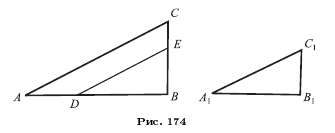
\includegraphics{mppics/ris-174}
\caption{}\label{1938/ris-174}
\end{figure}

Для доказательства применим тот же приём, которым мы пользовались ранее.
На $AB$ отложим $BD=A_1B_1$ и проведём $DE\parallel AC$.
Тогда получим вспомогательный $\triangle DBE$, подобный $\triangle ABC$.
Докажем, что он равен $\triangle A_1B_1C_1$.
Из подобия треугольников $ABC$ и $DBE$ следует:
\[\frac{AB}{DB}=\frac{AC}{DE}.\eqno(2)\]

Сравнивая эту пропорцию с данной (1), находим, что первые отношения их одинаковы;
следовательно, равны и вторые отношения, то есть 
\[\frac{AC}{DE}=\frac{AC}{A_1C_1},\]
откуда
\[DE=A_1C_1.\]

Теперь видим, что треугольники $BDE$ и $A_1B_1C_1$ имеют по равной гипотенузе и равному катету, следовательно, они равны;
а так как один из них подобен $\triangle ABC$, то и другой ему подобен.

\paragraph{}\label{1938/165}
\so{Теорема} (об отношении высот).
\textbf{\emph{В подобных треугольниках соответственные стороны пропорциональны соответственным высотам}}, то есть тем высотам, которые опущены на соответственные стороны.

\begin{figure}[h!]
\centering
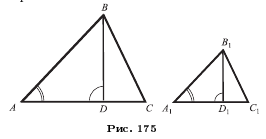
\includegraphics{mppics/ris-175}
\caption{}\label{1938/ris-175}
\end{figure}


Действительно, если треугольники $ABC$ и $A_1B_1C_1$ (рис.~\ref{1938/ris-175}) подобны, то прямоугольные треугольники $BAD$ и $B_1A_1D_1$ также подобны ($\angle A = \angle A_1$ и $\angle D=\angle D_1$);
поэтому:
\[\frac{BD}{B_1D_1}=\frac{AB}{A_1B_1}=\frac{BC}{B_1C_1}=\frac{AC}{A_1C_1}.\]
